% TAG -- Operating guide for running training.
% Self-contained: upload this single file to Overleaf and compile with pdfLaTeX.
\documentclass[11pt,a4paper]{article}

\usepackage[margin=2.4cm]{geometry}
\usepackage[T1]{fontenc}
\usepackage[utf8]{inputenc}
\usepackage{lmodern}
\usepackage{microtype}
\usepackage{xcolor}
\usepackage{listings}
\usepackage{booktabs}
\usepackage{enumitem}
\usepackage{tikz}
\usetikzlibrary{arrows.meta,positioning,fit,backgrounds}
\usepackage[colorlinks=true,linkcolor=blue!55!black,urlcolor=blue!55!black]{hyperref}

\definecolor{shellbg}{RGB}{245,246,248}
\definecolor{shellrule}{RGB}{205,210,216}
\definecolor{keyword}{RGB}{20,90,160}
\definecolor{comment}{RGB}{100,110,120}

\lstdefinestyle{shell}{
  basicstyle=\ttfamily\small,
  backgroundcolor=\color{shellbg},
  frame=single,
  rulecolor=\color{shellrule},
  framesep=6pt,
  xleftmargin=8pt,
  breaklines=true,
  breakatwhitespace=false,
  postbreak=\mbox{\textcolor{keyword}{$\hookrightarrow$}\space},
  columns=fullflexible,
  keepspaces=true,
  showstringspaces=false,
  commentstyle=\color{comment}\itshape,
  morecomment=[l]{\#},
}
\lstset{style=shell}

\newcommand{\cmd}[1]{\texttt{\small #1}}
\newcommand{\file}[1]{\texttt{\small #1}}
\newcommand{\topicname}[1]{\texttt{\small #1}}

\title{\textbf{TAG: Labyrinth Marble Robot}\\[2mm]
       \large Operating Guide --- Running a Training Session}
\author{}
\date{\today}

\begin{document}
\maketitle
\thispagestyle{empty}

\begin{center}
\begin{minipage}{0.9\textwidth}
\small\itshape
This guide covers how to run a reinforcement-learning training session on the TAG
labyrinth robot: what runs where, in what order, how to verify the system is
healthy before committing hours to a run, and what to do when it is not.
Everything here refers to the \file{tag\_*} workspace.
\end{minipage}
\end{center}
\vspace{4mm}

\tableofcontents
\newpage

%==========================================================================
\section{System overview}

Training is split across two machines. The \textbf{robot PC} is wired to the
labyrinth and handles perception and actuation in real time. The \textbf{server}
holds the GPU and runs the DreamerV3 learner. They exchange observations and
actions over a TCP socket.

\begin{center}
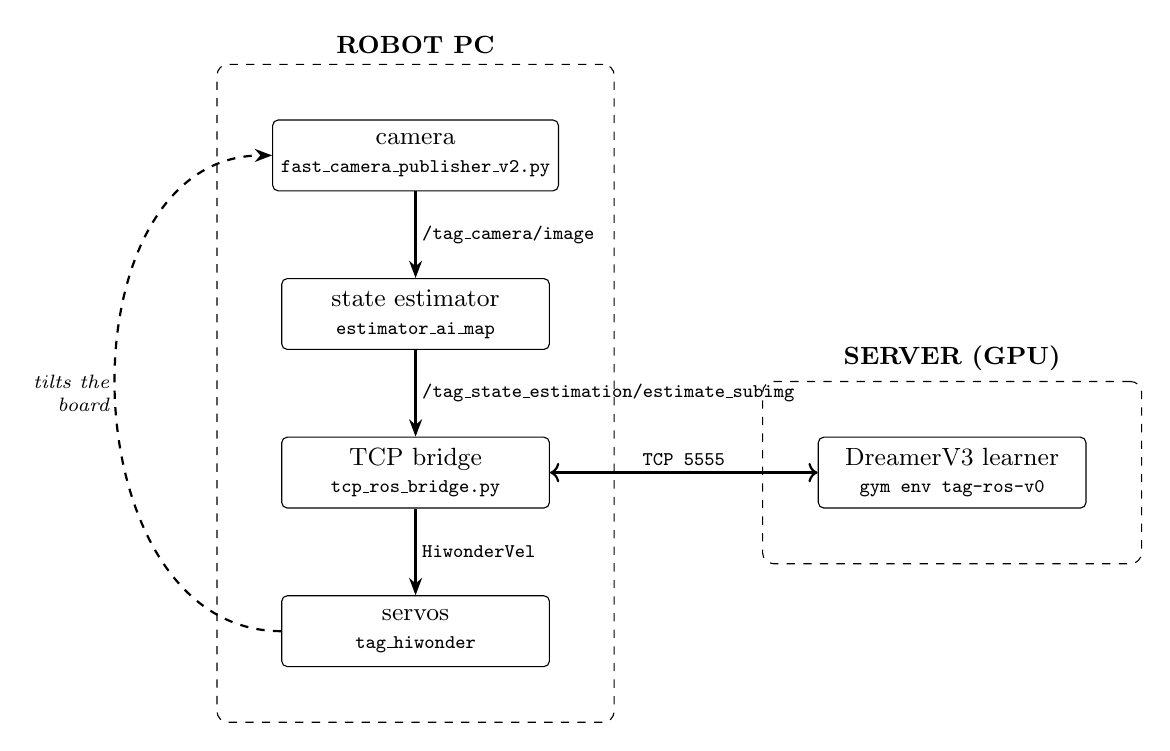
\begin{tikzpicture}[
  box/.style={draw, rounded corners=2pt, align=center, font=\small,
              minimum height=9mm, minimum width=34mm, inner sep=3pt, fill=white},
  lbl/.style={font=\scriptsize\ttfamily, inner sep=2pt},
  plain/.style={font=\scriptsize\itshape, inner sep=2pt},
  arr/.style={-{Stealth[length=2.2mm]}, thick}
]
\node[box] (cam) {camera\\[-1pt]{\scriptsize\ttfamily fast\_camera\_publisher\_v2.py}};
\node[box, below=11mm of cam] (est) {state estimator\\[-1pt]{\scriptsize\ttfamily estimator\_ai\_map}};
\node[box, below=11mm of est] (br)  {TCP bridge\\[-1pt]{\scriptsize\ttfamily tcp\_ros\_bridge.py}};
\node[box, below=11mm of br]  (sv)  {servos\\[-1pt]{\scriptsize\ttfamily tag\_hiwonder}};
\node[box, right=34mm of br]  (srv) {DreamerV3 learner\\[-1pt]{\scriptsize\ttfamily gym env tag-ros-v0}};

\draw[arr] (cam) -- node[lbl,right] {/tag\_camera/image} (est);
\draw[arr] (est) -- node[lbl,right] {/tag\_state\_estimation/estimate\_subimg} (br);
\draw[arr] (br)  -- node[lbl,right] {HiwonderVel} (sv);
\draw[arr,<->] (br) -- node[lbl,above] {TCP 5555} (srv);
% physical loop: the servos tilt the board, which the camera observes.
\draw[arr,dashed] (sv.west) to[out=180,in=180,looseness=1.15]
      node[plain,left,align=right,pos=0.5] {tilts the\\board} (cam.west);

\begin{scope}[on background layer]
  \node[draw, dashed, rounded corners, fit=(cam)(est)(br)(sv),
        inner sep=7mm, label={[font=\small\bfseries]above:ROBOT PC}] {};
  \node[draw, dashed, rounded corners, fit=(srv),
        inner sep=7mm, label={[font=\small\bfseries]above:SERVER (GPU)}] {};
\end{scope}
\end{tikzpicture}
\end{center}

\paragraph{What the estimator produces.}
A learned ONNX detector locates the marble in the image. Four blue dots on the
moving plate give a fresh pixel-to-metres homography every frame, so the map
follows the plate as it tilts; four dots on the fixed outer frame give the world
reference against which the tilt angles are measured. HSV colour thresholding is
used \emph{only} to track those eight dots, never as a fallback marble detector.

\paragraph{Ordering constraints.} Two, and both matter:
\begin{enumerate}[nosep,left=6mm]
  \item The \textbf{server must be running before the PC bridge}. The server's
        gym environment \emph{listens} on port 5555; the bridge connects out to
        it.
  \item The \textbf{camera must be running before the estimator}, which
        subscribes to \topicname{/tag\_camera/image}.
\end{enumerate}

%==========================================================================
\section{Prerequisites}

\begin{itemize}[nosep,left=6mm]
  \item \textbf{Robot PC:} Ubuntu 22.04, ROS~2 Humble, the TAG workspace built at
        \file{\~{}/CYBER/tag}. A See3CAM (or compatible V4L2) camera and two
        Hiwonder LX-16A servos over USB HID.
  \item \textbf{Server:} the TAG workspace synced to \file{\~{}/tag}, and a Python
        environment with JAX/CUDA, \cmd{gym}, \cmd{opencv-python},
        \cmd{numpy} and \cmd{ament\_index\_python}. The server needs
        \emph{neither} ROS nor colcon --- see Section~\ref{sec:server-notes}.
\end{itemize}

Verify the PC workspace resolves to the right packages before anything else:

\begin{lstlisting}
cd ~/CYBER/tag && source install/setup.bash
python3 -c "from ament_index_python.packages import get_package_share_directory as g; print(g('tag_state_estimation'))"
# expect a path under ~/CYBER/tag/install/
\end{lstlisting}

\textbf{Every PC terminal below needs the workspace sourced.} A stock shell does
not do this, so run \cmd{cd \~{}/CYBER/tag \&\& source install/setup.bash} first
in each one.

%==========================================================================
\section{Start-up sequence}
\label{sec:startup}

\subsection*{Step 0 --- stop anything already running}

Stale nodes hold the camera device and publish onto the same topics.

\begin{lstlisting}
pkill -f 'tcp_ros_bridge|hiwonder_compat|estimator_ai|fast_camera_publisher|overlay_map_view'
\end{lstlisting}

\subsection*{Step 1 --- server: start the learner}

\begin{lstlisting}
ssh <user>@<server>
cd ~/tag
TAG_LOGDIR=~/tag_logs/run1 ./run_server_dreamer_stuck_gpu0.sh
\end{lstlisting}

Use a fresh \cmd{TAG\_LOGDIR} for each run so checkpoints and replay chunks do
not mix. \textbf{Wait for this line before continuing:}

\begin{lstlisting}
[TCP ENV] Waiting for PC bridge on 0.0.0.0:5555 ...
\end{lstlisting}

Leave the terminal open; this process is the learner.

\subsection*{Step 2 --- PC: camera}

\begin{lstlisting}
cd ~/CYBER/tag && source install/setup.bash
python3 fast_camera_publisher_v2.py
\end{lstlisting}

Expect periodic \cmd{Publish FPS: \~{}40}. This script also locks white balance
and exposure, so the marble's colour stays stable across the board.

\subsection*{Step 3 --- PC: state estimator}

\begin{lstlisting}
cd ~/CYBER/tag && source install/setup.bash
./run_ai_map_estimator.sh
\end{lstlisting}

Every parameter defaults to its calibrated value, so pass nothing unless you
intend to override it. Add \cmd{-p show\_image:=true} for an annotated camera
window showing the tracked markers and marble.

\subsection*{Step 4 --- PC: servos}

\begin{lstlisting}
cd ~/CYBER/tag && source install/setup.bash
ros2 run tag_hiwonder hiwonder_compat_node.py
\end{lstlisting}

If the servos do not respond, the cause is almost always USB hidraw permissions
rather than anything in ROS:

\begin{lstlisting}
./scripts/reconnect_hiwonder.sh
\end{lstlisting}

\subsection*{Step 5 --- PC: bridge to the server}

\begin{lstlisting}
cd ~/CYBER/tag && source install/setup.bash
python3 tcp_ros_bridge.py <SERVER_IP> 5555
\end{lstlisting}

The server terminal should change to report that the PC bridge has connected. If
the server is not on the same LAN, tunnel the port and connect to localhost
instead:

\begin{lstlisting}
ssh -N -L 5555:127.0.0.1:5555 <user>@<server>   # leave running
python3 tcp_ros_bridge.py 127.0.0.1 5555
\end{lstlisting}

\subsection*{Step 6 --- place the marble}

Put the marble at the start position. Training begins once the server logs
step~0. The servos pause periodically to cool down, controlled by
\cmd{TAG\_REST\_AFTER\_SEC} and \cmd{TAG\_REST\_DURATION\_SEC}.

%==========================================================================
\section{Verify before committing to a long run}
\label{sec:verify}

A degraded estimator trains a degraded policy, and it fails quietly rather than
crashing. Two commands, in a spare sourced terminal:

\begin{lstlisting}
ros2 topic hz   /tag_state_estimation/estimate         # want ~40 Hz
ros2 topic echo /tag_state_estimation/status --once     # want: valid
\end{lstlisting}

\begin{table}[h]
\centering\small
\begin{tabular}{@{}lll@{}}
\toprule
\textbf{Observation} & \textbf{Meaning} & \textbf{Action} \\
\midrule
$\sim$40\,Hz, \cmd{valid} & healthy & proceed \\
$\sim$13\,Hz & QoS frame loss & see Section~\ref{sec:trouble} \\
\cmd{ai\_marble\_missing} & detector lost the marble & transient; check lighting \\
\cmd{moving\_markers\_timeout} & plate quad lost & usually extreme tilt \\
\cmd{fixed\_marker\_jump\_rejected} & marker substitution refused & re-run marker selection \\
\cmd{ai\_hole\_rejected\_N} & marble judged inside hole $N$ & expected on a real fall \\
\cmd{speed\_gate} & implausible marble speed & check for detector jitter \\
\bottomrule
\end{tabular}
\caption{Interpreting the estimator's \topicname{status} topic.}
\end{table}

It is also worth viewing the map once per session, especially after any layout
change, to confirm the waypoints match the physical maze:

\begin{lstlisting}
cd ~/CYBER/tag && source install/setup.bash
python3 overlay_map_view_simple.py
\end{lstlisting}

The status panel reports per-axis session extremes. Roll the marble into all four
walls and read them: symmetric overshoot on an axis indicates that axis's marker
spacing is wrong, whereas one end over by $d$ and the other short by $d$
indicates the marker-quad centroid is offset from the playable centre. The
extremes only reflect where the marble has actually been, so touch every wall
before drawing conclusions.

%==========================================================================
\section{Monitoring the run}

On the server:

\begin{lstlisting}
tensorboard --logdir ~/tag_logs --port 6006
\end{lstlisting}

Then forward the UI port from your laptop and open \url{http://localhost:6006}:

\begin{lstlisting}
ssh -N -L 6006:127.0.0.1:6006 <user>@<server>
\end{lstlisting}

The primary learning signal is \cmd{episode/score}, which should trend upward
over real-world hours. Also useful are the model losses and \cmd{fps}. If
TensorBoard is unavailable on the server, copy the event files down instead:

\begin{lstlisting}
rsync -az <user>@<server>:'~/tag_logs/run1/events.out.tfevents.*' ~/tag_logs/run1/
tensorboard --logdir ~/tag_logs
\end{lstlisting}

%==========================================================================
\section{Shutting down}

\begin{lstlisting}
# on the PC
pkill -f 'tcp_ros_bridge|hiwonder_compat|estimator_ai|fast_camera_publisher|overlay_map_view'
# on the server: Ctrl-C the learner
\end{lstlisting}

Checkpoints are written to \cmd{TAG\_LOGDIR} periodically
(\cmd{--run.save\_every}), so a clean interrupt loses at most the last interval.

%==========================================================================
\section{Troubleshooting}
\label{sec:trouble}

\paragraph{The marble blinks in and out of the overlay, but the detector clearly
sees it.} This is a QoS problem, not a detection problem. Camera frames are
$640\times400\times3 = 768$\,kB, which DDS fragments across many UDP datagrams.
Under \cmd{BEST\_EFFORT} reliability a single lost fragment discards the entire
frame with no retransmission, and the loss arrives in bursts. Measured on this
rig with the camera publishing 40.6\,Hz, a \cmd{BEST\_EFFORT} subscriber received
13.1\,Hz with stalls up to 1669\,ms --- leaving 45\% of wall-clock time inside a
gap longer than the overlay's 250\,ms staleness threshold --- while every frame
it \emph{did} receive was valid at 0.994 confidence. Switching that subscriber to
\cmd{RELIABLE} gives 38--43\,Hz with a 60\,ms worst case. The estimator and the
calibration tools already use \cmd{RELIABLE}; several auxiliary scripts in the
repository still do not.

\paragraph{The estimator says \cmd{valid} but positions look wrong.} Re-run
marker selection (Section~\ref{sec:markers}). The drawn crosses shifting a few
pixels off your clicks at start-up is \emph{correct} --- the guard snaps to the
true dot centroids on its first frame.

\paragraph{Markers drift away from the dots over a long session.} The fixed quad
is anchored to its calibrated position and re-seeds itself if it wanders, so this
should not recur; if it does, the anchor radius may be too generous for your
setup.

\paragraph{\cmd{select\_markers} appears to save but nothing changes.} It writes
to whichever workspace wins \cmd{AMENT\_PREFIX\_PATH}, and
\file{install/setup.bash} \emph{appends} rather than prepends --- so a workspace
sourced earlier takes precedence. The estimator logs the marker file it actually
loaded, with its modification time, at start-up. Read that line.

\paragraph{The server rejects \cmd{--configs tag}.} DreamerV3 may be
pip-installed elsewhere on the server and shadow the copy in \file{\~{}/tag}. The
launcher puts \file{\$PROJECT\_ROOT/dreamerv3} first on \cmd{PYTHONPATH} to
prevent this; verify with
\cmd{python3 -c "import dreamerv3; print(dreamerv3.\_\_file\_\_)"}.

%==========================================================================
\section{Calibration}

Three independent calibrations. Only the first is needed routinely.

\subsection{Markers --- whenever the camera or board moves}
\label{sec:markers}

This is the one calibration you will repeat. It tells the estimator where the
eight blue reference dots are, so it can start tracking them.

\paragraph{Before you start.} Two preconditions, both easy to miss:
\begin{enumerate}[nosep,left=6mm]
  \item \textbf{The camera must already be running} --- \cmd{select\_markers}
        subscribes to \topicname{tag\_camera/image} and shows you a live frame. If
        the window never appears, the camera is not publishing.
  \item \textbf{Level the plate first.} The tool says so on start-up, and the
        reason is concrete: your clicks become the tracker's seeds, and it will
        only acquire dots within roughly 14\,px of them. The moving dots travel
        about 15\,px across the full tilt range, so seeds captured at a large
        tilt can fall outside the acquisition window once the plate returns to
        level.
\end{enumerate}

\paragraph{Run it.}
\begin{lstlisting}
cd ~/CYBER/tag && source install/setup.bash
ros2 run tag_state_estimation select_markers
\end{lstlisting}

Click the eight dots in this order --- the on-screen banner reminds you:

\begin{center}\small
\begin{tabular}{@{}cll@{}}
\toprule
\textbf{Order} & \textbf{Label} & \textbf{Dot} \\
\midrule
1--4 & \cmd{F1}--\cmd{F4} & \emph{fixed} outer frame: lower-left, lower-right, upper-right, upper-left \\
5--8 & \cmd{M1}--\cmd{M4} & \emph{moving} plate: same order \\
\bottomrule
\end{tabular}
\end{center}

\noindent Keys: \cmd{u} or Backspace to undo the last click, \cmd{r} to restart,
\cmd{q} or Escape to abort. After the eighth click it saves \file{markers.csv},
prints the path it wrote to, and waits for a keypress before exiting.

\paragraph{Then rebuild}, so the installed share directory picks up the new file:
\begin{lstlisting}
colcon build --packages-select tag_state_estimation --symlink-install
\end{lstlisting}

\paragraph{Two things that look like mistakes but are not.}
\begin{itemize}[nosep,left=6mm]
  \item The fixed crosses sit \emph{outside} the moving ones horizontally but
        \emph{inside} them vertically. That is the real geometry of the two dot
        rectangles.
  \item When the estimator starts, the drawn crosses shift a few pixels off where
        you clicked. That is the tracker snapping onto the true dot centroids ---
        it is what should happen. Precision clicking is unnecessary.
\end{itemize}

\paragraph{Verify it took.} The estimator logs the marker file it actually loaded,
\emph{with its modification time}, on start-up. Read that line: if the timestamp
is not from your run, the file was written somewhere else. That happens because
\cmd{select\_markers} saves into whichever workspace wins
\cmd{AMENT\_PREFIX\_PATH}, and \file{install/setup.bash} \emph{appends} to it, so
a workspace sourced earlier in the shell takes precedence.

\subsection{Camera intrinsics}

Record while tilting, then fit offline. Offline is faster and avoids interactive
lag:

\begin{lstlisting}
python3 tools/record_frames.py --seconds 90 --out /tmp/calib_frames
# tilt the plate slowly through its full range on both axes while recording
python3 tools/calibrate_camera_holes.py --frames_dir /tmp/calib_frames
colcon build --packages-select tag_state_estimation --symlink-install
\end{lstlisting}

This uses the 21 maze holes as a planar calibration target: their metric
positions are known from the DXF layout, and the marker homography predicts where
each should appear, so correspondences are established before any blob detection
runs. \textbf{Check two numbers before installing the result:} RMS reprojection
error below 1\,px, and recovered camera height within 5\% of your measured
lens-to-plate distance. The tool warns on both. The output,
\file{pinhole\_calib.json}, is picked up automatically; without it the estimator
falls back to $f = 300$\,px and no distortion.

\subsection{Marker geometry --- only if positions appear scaled}

\begin{lstlisting}
python3 tools/measure_hole_layout.py --frames_dir /tmp/calib_frames   # verify
python3 tools/fit_marker_geometry.py  --frames_dir /tmp/calib_frames  # fit
\end{lstlisting}

The first checks that the layout file matches the installed maze. The second
jointly fits the marker spacing and the marker-plane height. These two
\emph{must} be fitted together: with the camera nearly overhead they are
algebraically degenerate, and only a range of plate tilts separates them. The fit
reports the camera's sweep across the board frame so you can judge whether it had
the leverage --- roughly $99\times90$\,mm is ample, a few millimetres is not.

%==========================================================================
\section{Configuration reference}

Set these on the \textbf{server}, where the reward and termination logic lives.
The launcher script sets sensible values for all of them.

\begin{table}[h]
\centering\small
\begin{tabular}{@{}ll@{}}
\toprule
\textbf{Variable} & \textbf{Purpose} \\
\midrule
\cmd{TAG\_LOGDIR} & checkpoint, replay and TensorBoard directory \\
\cmd{TAG\_REWARD\_ON\_FAIL} & penalty when the marble is lost \\
\cmd{TAG\_TIMEOUT\_STEPS}, \cmd{\_PENALTY} & episode cap and its penalty \\
\cmd{TAG\_ANTICHEAT\_MAX\_STEP\_M}, \cmd{\_PENALTY} & rejects implausible position jumps \\
\cmd{TAG\_STUCK\_WINDOW\_SEC}, \cmd{\_RADIUS\_M}, \cmd{\_PENALTY} & stuck-marble detection \\
\cmd{TAG\_BALL\_LOSS\_GRACE\_SEC} & grace before a loss counts \\
\cmd{TAG\_REST\_AFTER\_SEC}, \cmd{\_DURATION\_SEC} & servo cooldown schedule \\
\cmd{TAG\_TCP\_PORT} & must match the port given to the bridge \\
\bottomrule
\end{tabular}
\caption{Server-side environment variables.}
\end{table}

On the \textbf{PC}, \file{tcp\_ros\_bridge.py} reads
\cmd{TAG\_MAX\_CMD\_1}/\cmd{\_2} (servo command clamps) and
\cmd{TAG\_BALL\_LOST\_RESET\_FRAMES}. Key estimator parameters, all defaulting to
their calibrated values:

\begin{table}[h]
\centering\small
\begin{tabular}{@{}lll@{}}
\toprule
\textbf{Parameter} & \textbf{Default} & \textbf{Note} \\
\midrule
\cmd{publish\_legacy\_topics} & \cmd{true} & \cmd{false} publishes under \topicname{/tag\_ai\_map/*} \\
\cmd{ai\_confidence\_threshold} & 0.90 & \\
\cmd{marker\_plane\_height\_m} & 0.010 & dot plane above the play surface \\
\cmd{marble\_radius\_m} & 0.006 & \\
\cmd{marker\_acquire\_radius\_px} & 14.0 & one-shot marker acquisition window \\
\cmd{hole\_rejection\_enabled} & \cmd{true} & \\
\cmd{show\_image} & \cmd{false} & annotated camera window \\
\bottomrule
\end{tabular}
\caption{Estimator parameters worth knowing.}
\end{table}

%==========================================================================
\section{Notes on the server setup}
\label{sec:server-notes}

The server does not need ROS or colcon. The TCP gym environment imports no ROS
message types --- only \cmd{ament\_index\_python}, to locate its own share
directory --- so the only requirement is a Python package directory plus a small
ament index entry. Concretely, \file{\~{}/tag/install/tag\_dreamer} contains an
index marker, \file{package.xml}, the path \file{.pkl} files, and a symlink to the
package source. Nothing is compiled.

Consequently the server is updated by file sync, not by \cmd{git pull}:

\begin{lstlisting}
rsync -az --delete \
  --exclude build --exclude install --exclude log --exclude __pycache__ --exclude .git \
  ~/CYBER/tag/ <user>@<server>:~/tag/
\end{lstlisting}

Note \cmd{--exclude install}: that preserves the hand-built prefix described
above. If it is ever removed, recreate the index marker, the two \file{.pkl}
files, and the package symlink.

\paragraph{Shared machine.} The GPU box may be in use by others. The launcher
pins the learner to GPU~0 via \cmd{--jax.policy\_devices} and
\cmd{--jax.train\_devices}; check what is already running before assuming a device
is free.

\paragraph{Keep both sides in step.} The learner and the robot must agree on the
maze layout and the reward logic. After changing either, re-sync the server and
restart both ends. A mismatch here trains against a maze that is not the one on
the table, and produces no error message.

\end{document}
